\documentclass[tikz]{standalone}

\colorlet{FilledSurface}{blue!20}
\colorlet{FilledSurfaceGroupOne}{blue!20}
\colorlet{FilledSurfaceGroupTwo}{red!20}
\colorlet{FilledSurfaceGroupThree}{green!20}
\colorlet{FilledSurfaceGroupFour}{magenta!20}
\colorlet{FormulaBackground}{green!10}
\colorlet{FormulaFrame}{green}


\usetikzlibrary{calc, intersections, decorations.markings, angles}

\tikzset{
    mark rect/.style={
        decoration={markings, mark=at position 0.5 with {
            \draw[fill=white] (-6pt,-2pt) rectangle (6pt,2pt);
        }}, postaction={decorate}
    }
}

\begin{document}
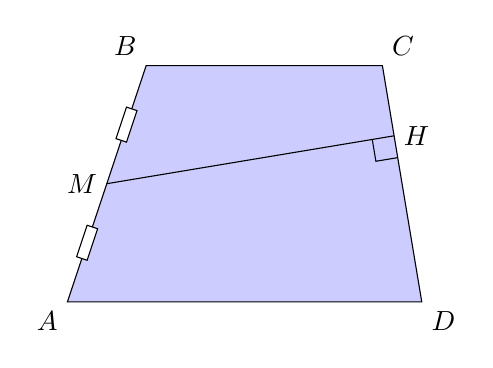
\begin{tikzpicture}

\coordinate (A) at (1, 0);
\coordinate (B) at (2, 3);
\coordinate (C) at (5, 3);
\coordinate (D) at (5.5, 0);

\coordinate (M) at ($(A)!0.5!(B)$);
\node[left] at (M) {$M$};

% Colorear superficies
\fill[FilledSurfaceGroupOne] (A) -- (B) -- (C) -- (D);

% Dibujamos los segmentos, luego de colorear las superficies para
% evitar que las superficies cubran a los segmentos.
\draw
(A) node [below left] {$A$} --
(B) node [above left] {$B$} --
(C) node [above right] {$C$} --
(D) node [below right] {$D$} -- cycle;

\path[mark rect] (A) -- (M);
\path[mark rect] (B) -- (M);

% Hallar proyección ortogonal de M sobre CD
\coordinate (H) at ($(C)!(M)!(D)$);
\draw (M) -- (H);
\node[right] at (H) {$H$};

\path pic [draw, angle radius = 8pt] {right angle = M--H--D};

\end{tikzpicture}
\end{document}
